
\documentclass{article}

\usepackage[ngerman]{babel}
\usepackage{graphicx}
\usepackage{indentfirst}
\usepackage{hyperref}
\usepackage{geometry}
\usepackage{changepage}
\usepackage{booktabs}
\usepackage{float}
\usepackage{tabulary}
\usepackage{xcolor}
\usepackage{multirow}

\graphicspath{ {./images/} }
\setlength\parindent{0pt}

\makeatletter
\newcommand{\sectionauthor}[1]{
	{\parindent 0em \large \scshape Autor: #1 \par \nobreak \vspace*{1em}}
	\@afterheading
}
\newcommand{\specification}[3]{
	{\parindent 0.5em \hangindent 3em \hypertarget{spec:#1:#2}{\textbf{/#1#2/}} #3 \par \nobreak \vspace*{0.5em}}
}
\makeatother

\title{Bibliotheksanwendung - Feinspezifikation}
\date{\today\\v1.0}
\author{
	Ivan Charviakou\\
	León Liehr\\
	Mohamad Najjar\\
	Jonas Picker\\
	Sergei Pravdin
}

\begin{document}
\maketitle
\begin{figure}[h]
	\centering
	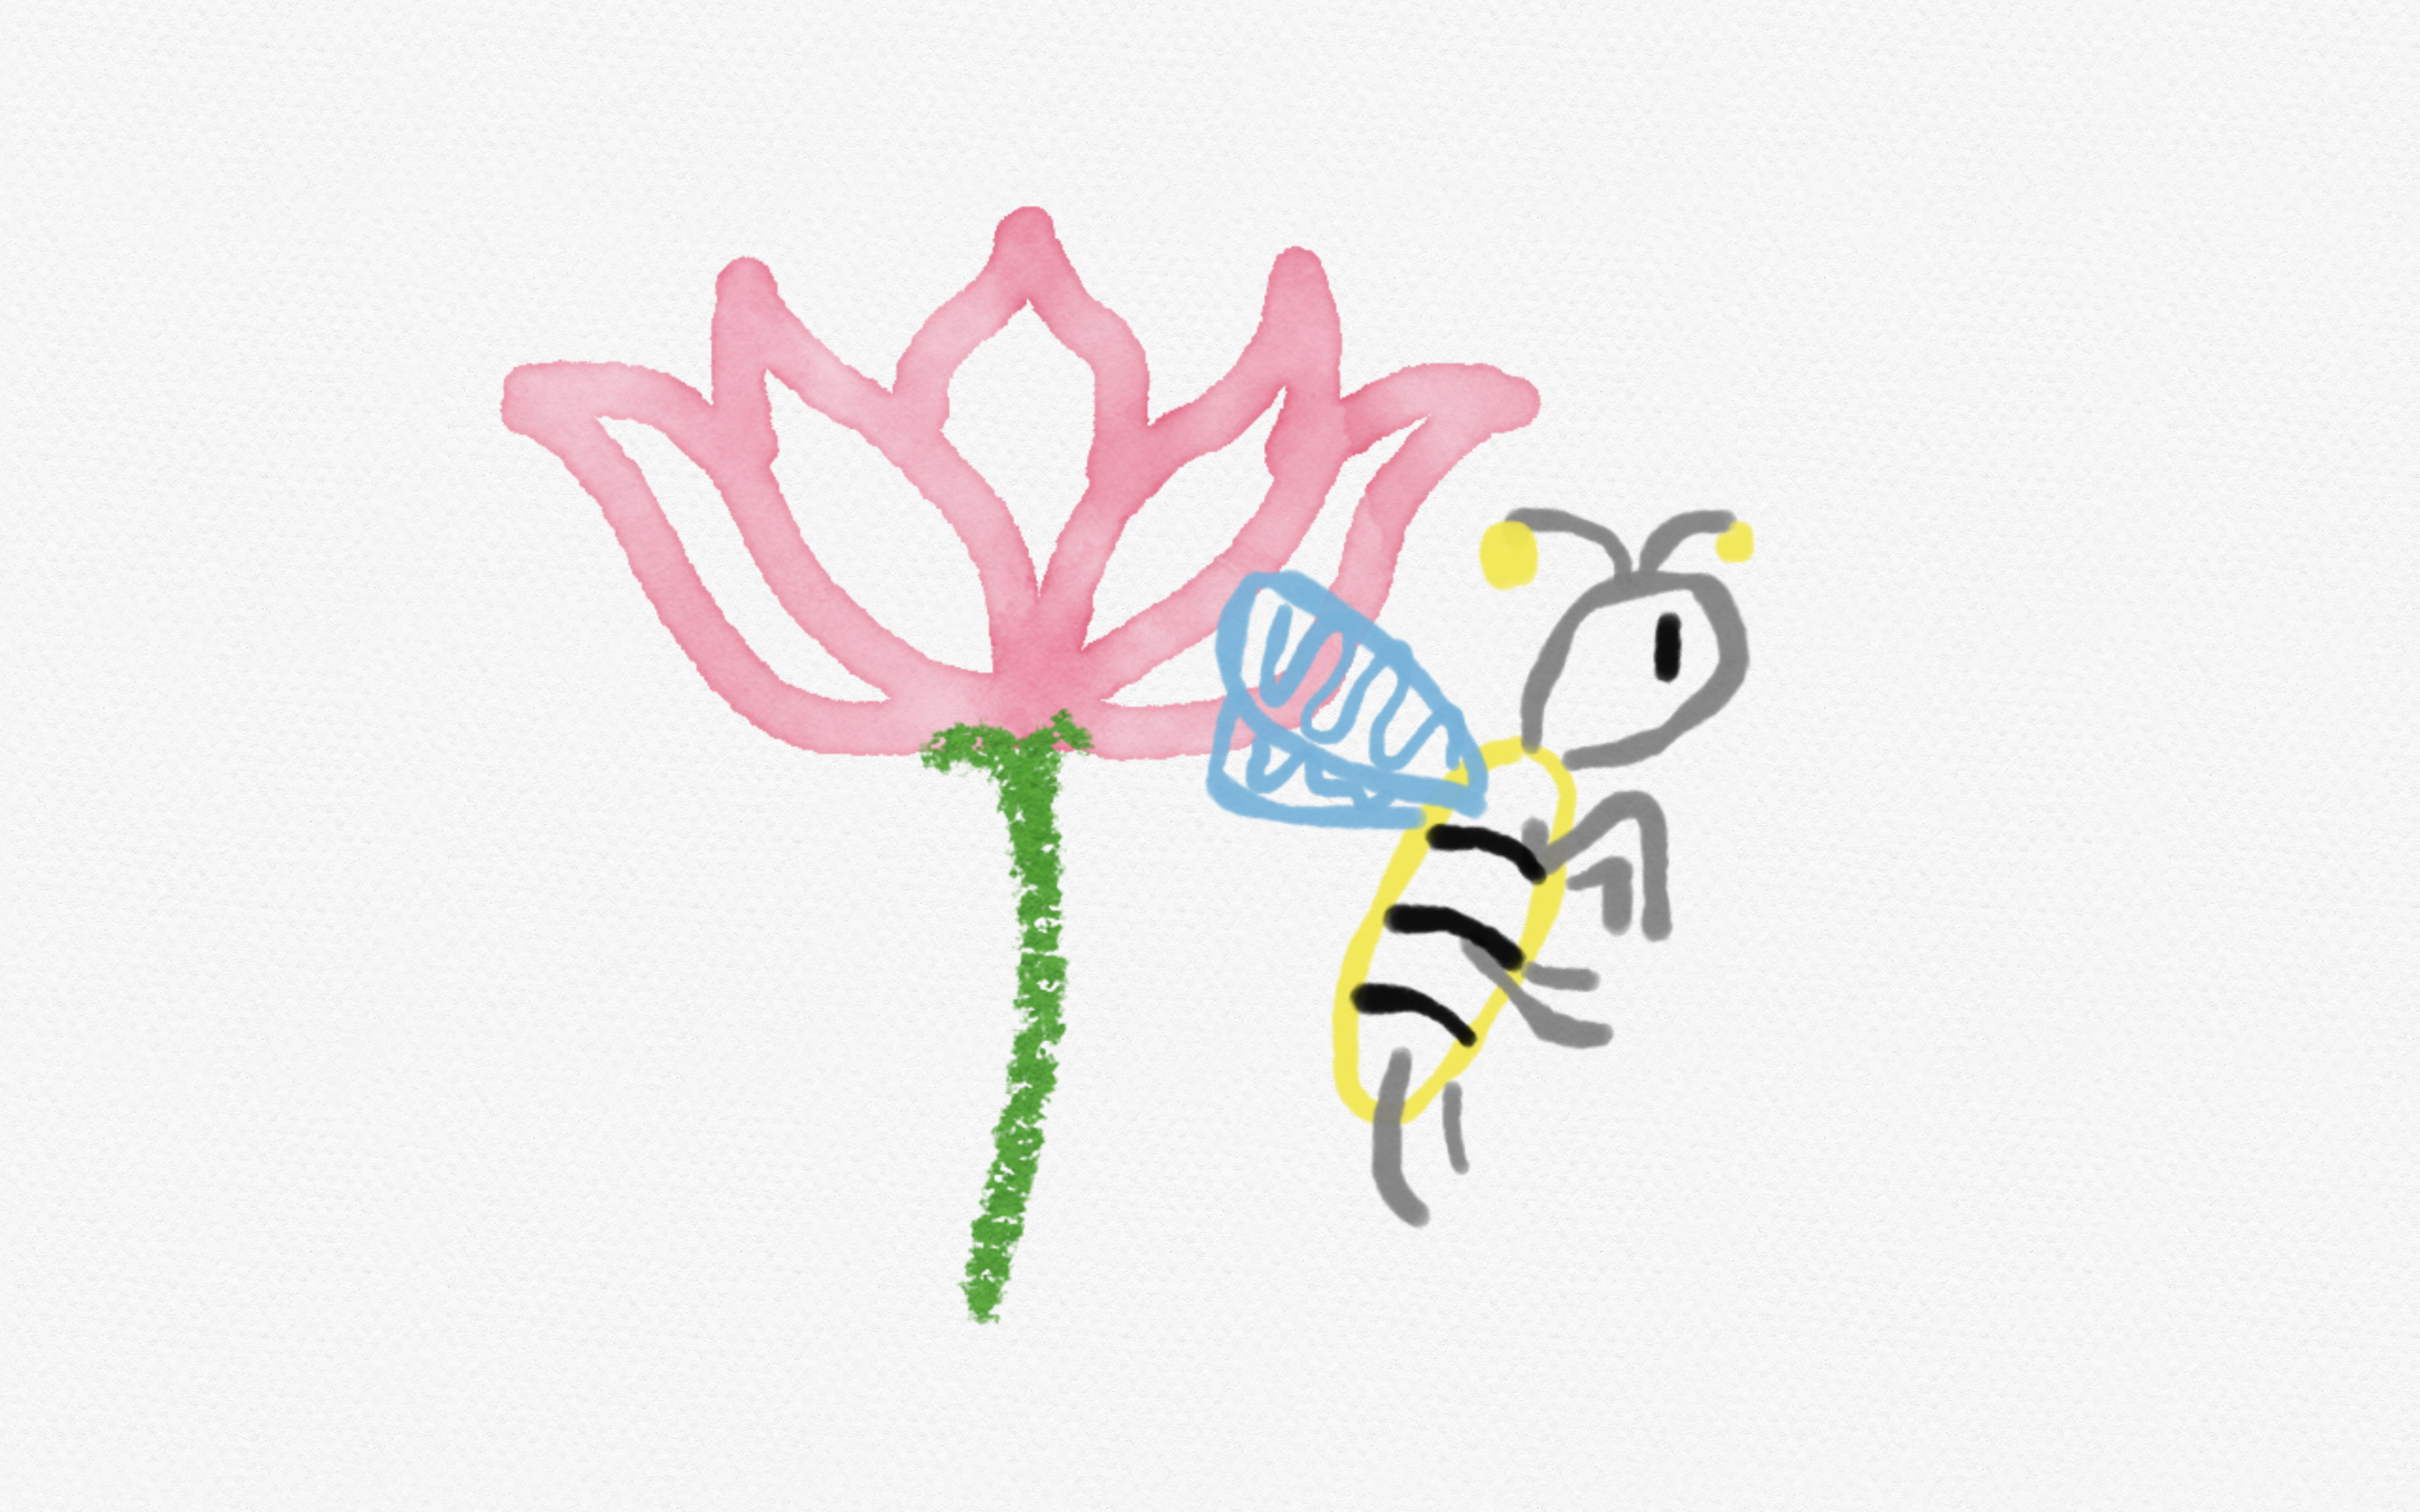
\includegraphics[width = 30em]{Logo}
\end{figure}
\newpage
\tableofcontents
\newpage

%----------------------------------------------------------------------Kapitel 1--------------------------------------------------------------------------------------------
\section{Einleitung}
Bei diesem Dokument handelt es sich um die Feinspezifikation unseres Bibliothekssystems. Es baut direkt auf dem vorangegangenen Entwurf auf und enthält einen noch genaueren Umriss der zu erstellenden Applikation.

%----------------------------------------------------------------------Kapitel 2--------------------------------------------------------------------------------------------


%----------------------------------------------------------------------Kapitel 3--------------------------------------------------------------------------------------------


%----------------------------------------------------------------------Kapitel 4--------------------------------------------------------------------------------------------


%----------------------------------------------------------------------Kapitel 5--------------------------------------------------------------------------------------------
\section{Systemkonfiguration}
Dieser Abschnitt beschreibt die Konfigurationsdatei und Sprachausgabe der Anwendung.
\subsection{Konfigurationsdatei}
Die Anwendung wird in einer Datei namens 'config' im \hyperlink{https://de.wikipedia.org/wiki/Java-Properties-Datei}{{\texttt.properties}-Format} konfiguriert. Diese Datei wird dann mit Funktionalitäten \hyperlink{https://docs.oracle.com/javase/7/docs/api/java/util/Properties.html}{dieser Klasse} eingelesen. Sie ist im Verzeichnis der Anwendung unter \texttt{/WebContent/WEB-INF/} zu finden und wird im Folgenden kurz beschrieben.
\subsubsection{Inhaltsbeschreibung}
Die mit \textcolor{green}{!} oder \textcolor{green}{\#} eingeleiteten Zeilen der Dateien enthalten Kommentare. Alle unmarkierten Zeilen halten ein Paar aus einem Schlüssel und einem mit \texttt{:} getrennten Wert. Nur die Werte dürfen verändert werden! 
\begin{center}
\begin{table}
\begin{tabular} {| c | c | c |}
\hline
Schlüsselname & Wertebeschreibung & Wertebereich \\
\hline
DB_HOST & Die URL (bzw. URI) unter der der Datenbankserver erreichbar ist.& Ein \hyperlink{https://datatracker.ietf.org/doc/html/rfc3986}{'Uniform Ressource Identifier'}\\
\hline
DB_PORT & Der Port unter dem der Server Anfragen entgegennimmt. & Eine ganze Zahl von 0 bis 65535.\\
\hline
DB_NAME & Der Name der Datenbank auf dem Server. & Ein String.\\
\hline
DB_USER & Der Name eines in der Datenbank registrierten Benutzers. & Ein String.\\
\hline
DB_PASSWORD & Das Passwort des obigen Benutzers. & Ein String. \\
\hline
DB_CAPACITY & Die maximale Anzahl an Verbindungen, die die Datenbank dem Server zu Verfügung stellen kann. & Eine natürliche Zahl (nicht 0).\\
\hline
MAILSERVER_HOST & Der URI unter der der E-Mail-Server erreichbar ist. &  Ein \hyperlink{https://datatracker.ietf.org/doc/html/rfc3986}{'Uniform Ressource Identifier'} \\ 
\hline
MAILSERVER_PORT & Der Port durch den Anfragen an den Server geleitet werden. & Eine ganze Zahl von 0 bis 65535. Typischer Standartwert ist 25. \\
\hline
MAIL_SOURCE &  & \\
\hline
SCAN_INTERVAL &  & \\
\hline
DEFAULT_ADMIN_MAIL &  & \\
\hline
LOG_LEVEL &  & \\
\hline
LOG_CONSOLE &  & \\
\hline
 & & \\
\hline
\end{tabular}
\end{table}
\end{center}
 
\subsubsection{Prototyp}
\subsection{Sprachressourcen}

%----------------------------------------------------------------------Kapitel 6--------------------------------------------------------------------------------------------


%----------------------------------------------------------------------Kapitel 7--------------------------------------------------------------------------------------------
\section{Datenbankschema}
\subsection{}
\subsection{}
\subsection{}

%----------------------------------------------------------------------Kapitel 8--------------------------------------------------------------------------------------------


%----------------------------------------------------------------------Kapitel 9--------------------------------------------------------------------------------------------
\section{Sicherheit}

\subsection{Injections}

\subsection{Insecure Direct Object References}

\subsection{Session Fixation}

\subsection{Userinput}

\subsection{System Secrecy}
\end{document}